\documentclass{article}

\usepackage{amsmath}
\usepackage{amsfonts} % For math fonts.
\usepackage{amssymb} % For other math symbols not covered by amsmath.
\usepackage[pdftex]{graphicx} % For pictures, use \includegraphics[scale=decimal]{pic.png}; must be a .png file type.
\usepackage{multicol}
\usepackage{textcomp}
\usepackage[colorlinks = true, urlcolor = blue]{hyperref}
\usepackage{enumitem}
\usepackage{graphbox} 
\usepackage{subfig}
\usepackage{multicol}
\usepackage{nopageno}
\usepackage{bm}


\usepackage{tikz}
\usetikzlibrary{positioning, calc}
\usetikzlibrary{shapes.geometric,angles,quotes}
\usepackage{tikz-3dplot}


%page formatting
\usepackage{fullpage}
\setlength{\parindent}{0pt}


\newcommand{\tab}{\hspace*{0.25in}}
\newcommand{\csq}[1]{\reflectbox{''}#1''}  %This produces CS style quotes.
\newcommand{\csqt}[1]{\text{\reflectbox{''}#1''}}  %This produces CS style quotes as text.


\usepackage{listings}
\lstset
{ %Formatting for code in appendix
    language=Python,
    basicstyle=\footnotesize,
    numbers=left,
    stepnumber=1,
    showstringspaces=false,
    tabsize=2,
    breaklines=true,
    breakatwhitespace=false,
}


\begin{document}



%split_point

%\end{document}
Lone Star \hfill Branching quiz\\
section 4\\
\begin{enumerate}
\item (3.1)  
		Use the following code to answer the below questions\\
		\mbox{ \hspace*{0.25in}	\lstinputlisting[language=Python]{./code/c1.py}}
		\begin{enumerate}
			\item Find four values of my\_var so each of the four assignment statements will be executed: 
				each value should cause one assignment statement to be executed.
			\item Find four ranges of my\_var values that will cause each of the four assignment 
				statements to be executed.
		\end{enumerate}


\item (3.2)  
		In Harry Potter, the currency consists of knuts, sickle, and galleon.  There are 29 knuts in 
		one sickle and 17 sickles in one galleon.  Write a program that will convert some amount of 
		knuts into the fewest amount of coins possible.  Only print non-zero values, meaning don't 
		print something similar to ``0 sickles.''  For example,
		\begin{itemize}
			\item Given 32 knuts, output 1 sickle 3 knuts
			\item Given 544 knuts, output 1 galleon 4 sickles 18 knuts
			\item Given 993 knuts, output 2 galleons 7 knuts. 
				Do \textbf{not} output 2 galleons 0 sickle 7 knuts.
		\end{itemize}




\item (3.3)  
		The table below shows the maximum health of characters based on race and class for a new 
		video game I am creating.  Write a program that asks the user for the race and the class of 
		their character, and then sets the \textit{health\_points}	variable according to the table 
		below.
		\begin{flushright}
		\begin{tabular}{c|cc}
			& \multicolumn{2}{c}{Race}\\
			Class & Elf & Ogre \\ \hline
			Warrior & 150 & 200\\
			Bard & 75 & 100\\
			Wizard & 25 & 50 \\
		\end{tabular}
		\end{flushright}
		
		\vspace*{-6em}
		\textit{health\_points} = -1\\
		\#Your code here.
		\vspace*{3em}





\end{enumerate}
\pagebreak
Dot Matrix \hfill Branching quiz\\
section 5\\
\begin{enumerate}
\item (3.1)  
		Write a program that prompts the user for a letter and checks whether the letter is a vowel 
		or consonant.  A vowel should output \textit{\csq{vowel}}, and a consonant should output 
		\textit{consonant}.  You may assume only lower case letters. Below is sample output.\\
		Hint: In the English language, a, e, i, o, and u are the vowels.
	
		\begin{figure}[h]
		\centering
			\begin{minipage}{.5\textwidth}
			\centering
				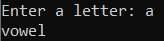
\includegraphics[scale=1.2]{./imgs/vowelYesAlt.png}
			\end{minipage}%
				%
			\begin{minipage}{.5\textwidth}
			\centering
				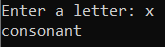
\includegraphics[scale=1.1]{./imgs/vowelNoAlt.png}
			\end{minipage}
		\end{figure}





\item (3.2)  
		%https://edabit.com/challenge/sfqudQHQ3HPpd7dZb
		Create a game of Rock, Paper, Scissors that takes user inputs.  
		The first input should be player 1 and the second 
		input should be player 2.  Print the winner according to the following rules. 
		\begin{itemize}
			\item Rock beats Scissors
			\item Scissors beats Paper
			\item Paper beats Rock
		\end{itemize}		
		For example:

		\hfill 
		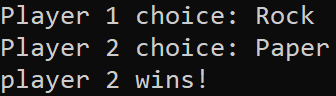
\includegraphics[height = 0.5in]{./imgs/RockPaperScissors1.PNG} \hfill 
		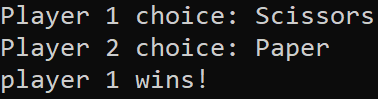
\includegraphics[height = 0.5in]{./imgs/RockPaperScissors2.PNG} \hfill  
		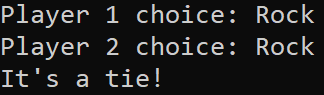
\includegraphics[height = 0.5in]{./imgs/RockPaperScissors3.PNG} \hfill \ 


\item (3.3)  
		The table below show what your resting heart rate should be based on age and athleticism.  
		Write a program that asks the user their age and desired athleticism goal, and then outputs 
		what their resting heart rate should be.

		\begin{minipage}{.45\textwidth}
			\begin{tabular}{c|cc}
				& \multicolumn{2}{c}{Athleticism}\\
				Age & Above Average & Below Average \\ \hline
				20 -- 39 & 47 -- 72 & 73 -- 93\\
				40 -- 59 & 46 -- 71 & 72 -- 94\\
				60 -- 79 & 45 -- 70 & 71 -- 97 \\
			\end{tabular}
		\end{minipage}
		\begin{minipage}{.45\textwidth}
			\vspace*{1em}
			Your end output should look similar to this
			\fbox{\parbox{\textwidth}{ Enter your age: 45\\
			Enter your athleticism goal: Below Average\\
			Your resting heart rate should be between 72--94.}}
		\end{minipage}





\end{enumerate}
\pagebreak
Dark Helmet \hfill Branching quiz\\
section 4\\
\begin{enumerate}
\item (3.1)  
		Write a program that asks the user for three numbers, and then determines (and outputs)
		which of the numbers is the smallest.  Do not use the built-in function \textit{min}().\\
		For example, \\ \ \hfill
		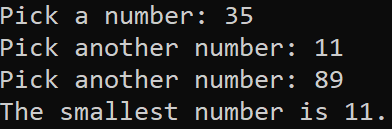
\includegraphics[height = 0.6in]{./imgs/smallest_ex1.PNG} \hfill
		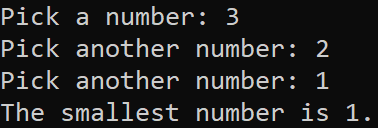
\includegraphics[height = 0.6in]{./imgs/smallest_ex2.PNG} \hfill \ 




\item (3.2)  
		Primary U.S. interstate highways are numbered 1-99.  Odd numbers (like 5 or 95) go north/
		south, and evens (like 10 or 82) go east/west.  Auxiliary highways are numbered 100-999, and 
		service the primary highway indicated by the rightmost two digits.  Thus, I-405 services 
		I-5, and I-290 services I-90.
		
		Note: 200 is not a valid auxiliary highway because 00 is not a valid primary highway 
		number.\\
		
		Let the user pick a highway number.  Given a valid highway number, indicate whether it runs 
		north/south or east/west.  If it is an invalid highway number, indicate that it is an 
		invalid highway number. \\
		For example,
		
		\hfill
		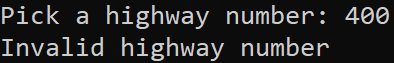
\includegraphics[width = 2in]{./imgs/highwayValidator1.PNG} \hfill
		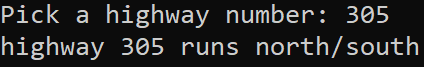
\includegraphics[width = 2in]{./imgs/highwayValidator2.PNG} \hfill \ 

		\hfill 
		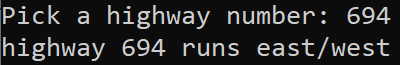
\includegraphics[width = 2in]{./imgs/highwayValidator3.PNG} \hfill 
		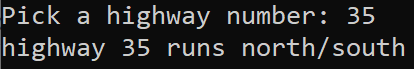
\includegraphics[width = 2in]{./imgs/highwayValidator4.PNG} \hfill \ 



\item (3.3)  
		The table below shows the maximum health of characters based on race and class for a new 
		video game I am creating.  Write a program that asks the user for the race and the class of 
		their character, and then sets the \textit{health\_points}	variable according to the table 
		below.
		\begin{flushright}
		\begin{tabular}{c|cc}
			& \multicolumn{2}{c}{Race}\\
			Class & Elf & Ogre \\ \hline
			Warrior & 150 & 200\\
			Bard & 75 & 100\\
			Wizard & 25 & 50 \\
		\end{tabular}
		\end{flushright}
		
		\vspace*{-6em}
		\textit{health\_points} = -1\\
		\#Your code here.
		\vspace*{3em}





\end{enumerate}
\pagebreak
President Skroob \hfill Branching quiz\\
section 1\\
\begin{enumerate}
\item (3.1)  
		Write a program that prompts the user for a letter and checks whether the letter is a vowel 
		or consonant.  A vowel should output \textit{\csq{vowel}}, and a consonant should output 
		\textit{consonant}.  You may assume only lower case letters. Below is sample output.\\
		Hint: In the English language, a, e, i, o, and u are the vowels.
	
		\begin{figure}[h]
		\centering
			\begin{minipage}{.5\textwidth}
			\centering
				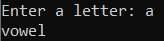
\includegraphics[scale=1.2]{./imgs/vowelYesAlt.png}
			\end{minipage}%
				%
			\begin{minipage}{.5\textwidth}
			\centering
				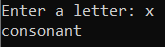
\includegraphics[scale=1.1]{./imgs/vowelNoAlt.png}
			\end{minipage}
		\end{figure}





\item (3.2)  
		Primary U.S. interstate highways are numbered 1-99.  Odd numbers (like 5 or 95) go north/
		south, and evens (like 10 or 82) go east/west.  Auxiliary highways are numbered 100-999, and 
		service the primary highway indicated by the rightmost two digits.  Thus, I-405 services 
		I-5, and I-290 services I-90.
		
		Note: 200 is not a valid auxiliary highway because 00 is not a valid primary highway 
		number.\\
		
		Let the user pick a highway number.  Given a valid highway number, indicate whether it runs 
		north/south or east/west.  If it is an invalid highway number, indicate that it is an 
		invalid highway number. \\
		For example,
		
		\hfill
		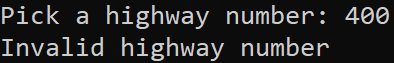
\includegraphics[width = 2in]{./imgs/highwayValidator1.PNG} \hfill
		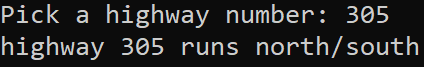
\includegraphics[width = 2in]{./imgs/highwayValidator2.PNG} \hfill \ 

		\hfill 
		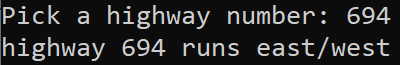
\includegraphics[width = 2in]{./imgs/highwayValidator3.PNG} \hfill 
		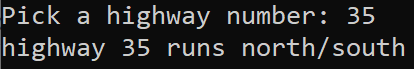
\includegraphics[width = 2in]{./imgs/highwayValidator4.PNG} \hfill \ 



\item (3.3)  
		The table below shows the maximum health of characters based on race and class for a new 
		video game I am creating.  Write a program that asks the user for the race and the class of 
		their character, and then sets the \textit{health\_points}	variable according to the table 
		below.
		\begin{flushright}
		\begin{tabular}{c|cc}
			& \multicolumn{2}{c}{Race}\\
			Class & Elf & Ogre \\ \hline
			Warrior & 150 & 200\\
			Bard & 75 & 100\\
			Wizard & 25 & 50 \\
		\end{tabular}
		\end{flushright}
		
		\vspace*{-6em}
		\textit{health\_points} = -1\\
		\#Your code here.
		\vspace*{3em}





\end{enumerate}
\pagebreak
\end{document}